% Choose one to switch between slides and handout
%\documentclass[]{beamer}
\documentclass[handout]{beamer}

% Video Meta Data
\title{Smart Contracts and Decentralized Finance Applications}
\subtitle{Gas and Fees}
\author{Prof. Dr. Fabian Schär}
\institute{University of Basel}

% Config File
% Packages
\usepackage[utf8]{inputenc}
\usepackage{hyperref}
\usepackage{gitinfo2}
\usepackage{tikz}
 \usetikzlibrary{calc}
\usepackage{amsmath}
\usepackage{mathtools}
\usepackage{bibentry}
\usepackage{xcolor}
\usepackage{colortbl} % Add colour to LaTeX tables
\usepackage{caption}
\usepackage[export]{adjustbox}
\usepackage{pgfplots} \pgfplotsset{compat = 1.17}
\usepackage{makecell}
\usepackage{fancybox}
\usepackage{ragged2e}
\usepackage{fontawesome}
\usepackage{seqsplit}
\usepackage{tabularx}
\usepackage{tcolorbox}
\usepackage{booktabs} % use instead  \hline in tables

% Color Options
\definecolor{highlight}{rgb}{0.65,0.84,0.82}
\definecolor{focus}{rgb}{0.72, 0, 0}
\definecolor{lightred}{rgb}{0.8,0.5,0.5}
\definecolor{midgray}{RGB}{190,195,200}

 %UniBas Main Colors
\definecolor{mint}{RGB}{165,215,210}
\definecolor{anthracite}{RGB}{45,55,60}
\definecolor{red}{RGB}{210,5,55}

 %UniBas Color Palette (for graphics)
\definecolor{strongmint}{RGB}{30,165,165}
\definecolor{darkmint}{RGB}{0,110,110}
\definecolor{softanthracite}{RGB}{140,145,150}
\definecolor{brightanthracite}{RGB}{190,195,200}
\definecolor{softred}{RGB}{235,130,155}

%Custom Colors
\definecolor{lightergray}{RGB}{230, 230, 230}



% Beamer Template Options
\beamertemplatenavigationsymbolsempty
\setbeamertemplate{footline}[frame number]
\setbeamercolor{structure}{fg=black}
\setbeamercolor{footline}{fg=black}
\setbeamercolor{title}{fg=black}
\setbeamercolor{frametitle}{fg=black}
\setbeamercolor{item}{fg=black}
\setbeamercolor{}{fg=black}
\setbeamercolor{bibliography item}{fg=black}
\setbeamercolor*{bibliography entry title}{fg=black}
\setbeamercolor{alerted text}{fg=focus}
\setbeamertemplate{items}[square]
\setbeamertemplate{enumerate items}[default]
\captionsetup[figure]{labelfont={color=black},font={color=black}}
\captionsetup[table]{labelfont={color=black},font={color=black}}

\setbeamertemplate{bibliography item}{\insertbiblabel}

%tcolor boxes
\newtcolorbox{samplecode}[2][]{
  colback=mint, colframe=darkmint, coltitle=white,
  fontupper = \ttfamily\scriptsize, fonttitle= \bfseries\scriptsize,
  boxrule = 0mm, arc = 0mm,
  boxsep = 1.3mm, left = 0mm, right = 0mm, top = 0.5mm, bottom = 0mm, middle=0mm,
  #1,title=#2}
  
\newtcolorbox{keytakeaway}[2][]{
  colback=softred, colframe=red, coltitle=white,
  fontupper = \scriptsize, fonttitle= \bfseries\scriptsize,
  boxrule = 0mm, arc = 0mm,
  boxsep = 1.3mm, left = 0mm, right = 0mm, top = 0.5mm, bottom = 0mm, middle=0mm,
  #1,title=#2}

\newtcolorbox{exercise}[2][]{
  colback=brightanthracite, colframe=anthracite, coltitle=white,
  fontupper = \scriptsize, fonttitle= \bfseries\scriptsize,
  boxrule = 0mm, arc = 0mm,
  boxsep = 1.3mm, left = 0mm, right = 0mm, top = 0.5mm, bottom = 0mm, middle=0mm,
  #1,title=#2}



% Link Icon Command 
\newcommand{\link}{%
    \tikz[x=1.2ex, y=1.2ex, baseline=-0.05ex]{%
        \begin{scope}[x=1ex, y=1ex]
            \clip (-0.1,-0.1)
                --++ (-0, 1.2)
                --++ (0.6, 0)
                --++ (0, -0.6)
                --++ (0.6, 0)
                --++ (0, -1);
            \path[draw,
                line width = 0.5,
                rounded corners=0.5]
                (0,0) rectangle (1,1);
        \end{scope}
        \path[draw, line width = 0.5] (0.5, 0.5)
            -- (1, 1);
        \path[draw, line width = 0.5] (0.6, 1)
            -- (1, 1) -- (1, 0.6);
        }
    }

% Other commands
\newcommand\tab[1][0.5cm]{\hspace*{#1}} % for code boxes


% Read Git Data from Github Actions Workflow
% Defaults to gitinfo2 for local builds
\IfFileExists{gitInfo.txt}
	{\input{gitInfo.txt}}
	{
		\newcommand{\gitRelease}{(Local Release)}
		\newcommand{\gitSHA}{\gitHash}
		\newcommand{\gitDate}{\gitAuthorIsoDate}
	}

% Custom Titlepage
\defbeamertemplate*{title page}{customized}[1][]
{
  \vspace{-0cm}\hfill\includegraphics[width=2.5cm]{../config/logo_cif}
  \includegraphics[width=1.9cm]{../config/seal_wwz}
  \\ \vspace{2em}
  \usebeamerfont{title}\textbf{\inserttitle}\par
  \usebeamerfont{title}\usebeamercolor[fg]{title}\insertsubtitle\par  \vspace{1.5em}
  \small\usebeamerfont{author}\insertauthor\par
  \usebeamerfont{author}\insertinstitute\par \vspace{2em}
  \usebeamercolor[fg]{titlegraphic}\inserttitlegraphic
    \tiny \noindent \texttt{Release Ver.: \gitRelease}\\ 
    \texttt{Version Hash: \gitSHA}\\
    \texttt{Version Date: \gitDate}\\ \vspace{1em}
    
    
    \iffalse
  \link \href{https://github.com/cifunibas/Bitcoin-Blockchain-Cryptoassets/blob/main/slides/intro.pdf}
  {Get most recent version}\\
  \link \href{https://github.com/cifunibas/Bitcoin-Blockchain-Cryptoassets/blob/main/slides/intro.pdf}
  {Watch video lecture}\\ 
  
  \fi
  
  \vspace{1em}
  License: \texttt{Creative Commons Attribution-NonCommercial-ShareAlike 4.0 International}\\\vspace{2em}
  \includegraphics[width = 1.2cm]{../config/license}
}


% tikzlibraries
\usetikzlibrary{decorations.pathreplacing}
\usetikzlibrary{decorations.markings}
\usetikzlibrary{positioning}
\usetikzlibrary{calc}
\captionsetup{font=footnotesize}

%%%%%%%%%%%%%%%%%%%%%%%%%%%%%%%%%%%%%%%%%%%%%%
%%%%%%%%%%%%%%%%%%%%%%%%%%%%%%%%%%%%%%%%%%%%%%
\begin{document}

\thispagestyle{empty}
\begin{frame}[noframenumbering]
	\titlepage
\end{frame}

%%%	
\begin{frame}{The Halting Problem and its Implications}
\begin{columns}
	\begin{column}{0.25\textwidth}
		\center
		\includegraphics[width=\textwidth ]{../assets/images/alan-turing.png}
	\end{column}
	\begin{column}{0.65\textwidth}
		In 1936, Alan Turing has shown that a (turing) machine cannot tell if a script will halt or run forever, before execution.\\
		\vspace{1em}
		\link \href{https://www.cs.virginia.edu/~robins/Turing_Paper_1936.pdf}{Online PDF}\\
		\vspace{1em}	
		\uncover<2->{$\Rightarrow$ Infinite loops or resource intensive scripts are a potential attack vector that must be addressed.}\\
	\end{column}
\end{columns}

\vspace{1.0 em}
\uncover<3->{
	\begin{keytakeaway}{Bitcoin and Ethereum Deal With This Problem in Different Ways}
		\begin{itemize}
			\item Bitcoin Script is a deliberately limited scripting language.
			\item Ethereum has a Turing complete instruction set. It charges a small fee (gas) for each computation step.
		\end{itemize}
	\end{keytakeaway}
}
\end{frame}
%%%

%%%
\begin{frame}{Ethereum Gas Fees: The Basics}

Each EVM operation consumes a defined amount of gas. The user cannot change these amounts. Some examples:\footnote{\href{https://docs.google.com/spreadsheets/d/1m89CVujrQe5LAFJ8-YAUCcNK950dUzMQPMJBxRtGCqs}{Full list} \link}
	\begin{columns}
	\uncover<2->{
		\begin{column}{0.08\textwidth}
		\end{column}
		\begin{column}{0.25\textwidth}
			\begin{samplecode}{Addition}
				\begin{center}
					\includegraphics[width=2em]{../assets/images/plus.png}
				\end{center}
				$\rightarrow$ 3 gas units 
			\end{samplecode}				
		\end{column}
	}
	\uncover<3->{
		\begin{column}{0.25\textwidth}
			\begin{samplecode}{Multiplication}
				\begin{center}
					\includegraphics[width=2em]{../assets/images/multiply.png}
				\end{center}
				$\rightarrow$ 5 gas units 
			\end{samplecode}
		\end{column}
	}
	\uncover<4->{
		\begin{column}{0.25\textwidth}
			\begin{samplecode}{Store 256 bits}
				\begin{center}
					\includegraphics[width=2em]{../assets/images/database.png}
				\end{center}
				$\rightarrow$ 20k gas units 
			\end{samplecode}	
		\end{column}
	}
		\begin{column}{0.02\textwidth}
		\end{column}
	\end{columns}
\vspace{1em}

\uncover<5->{
For each transaction the user specifies a \textbf{gas limit}, i.e., the maximum amount of gas that can be consumed by it. Examples:
		\hspace{-1em}
		\begin{itemize}
			\item $21k$ gas units are required to send ETH.
			\item Gas consumption of contract execution varies.
		\end{itemize}
}
\vspace{0.5em}
\uncover<6->{
The user also sets the \textbf{gas price} for each transaction, i.e., the price in $\mu ETH$ or gwei the user offers to pay per unit of gas.
}

\end{frame}
%%%

%%%
\begin{frame}{Understanding the Ethereum Fee Process}

\vspace{-1.0 em}
	\begin{center}
	\begin{tikzpicture}
		\begin{footnotesize}
	\tiny
	\uncover<1->{
		\node (avatar1) at (-4.5, 5) {\includegraphics[width=.15\textwidth]{../assets/images/avatar.png}};
		\node (initiation) at (-0.5, 5) [circle,inner sep=-1pt,fill=mint, label={east,red:remainingGas = gasLimit}] {\begin{tabular}{l}Transaction\\Initiation \end{tabular}};
		\draw[->, dotted, very thick] (avatar1) -- (initiation) node[midway, below] (text1) {\begin{tabular}{l} User places amount\\ in GWEI equal to\\ gasLimit $\cdot$ gasPrice\\ in transactionEscrow\end{tabular}};
	}
	\uncover<2->{
		\node (remainingGas) at (-0.5,2.5) [diamond,fill=mint,aspect=2] {\begin{tabular}{l} Remaining\\ gas = 0 or\\ insufficient? \end{tabular}};
		\draw[->, dotted, very thick] (initiation) -- (remainingGas) node[midway, right] (text2) {};
	}
	\uncover<3->{
		\node (executeOperation) at (-0.5,0.5) [rectangle,fill=mint,minimum height=0.6cm, label={east,red:remainingGas = remainingGas - opCost}] {Execute Operation};
		\draw[->, dotted, very thick] (remainingGas) -- (executeOperation) node[midway, right] (text3) {no};
	}
	\uncover<4->{
		\node (remainingOperations) at (-0.5,-1.2) [diamond,fill=mint,aspect=2,minimum width=0.6cm] {\begin{tabular}{l} Remaining\\ Operations? \end{tabular}};
		\draw[->, dotted, very thick] (executeOperation) -- (remainingOperations) node[midway, right, mint] (text4) {};
	}
	\uncover<5->{
		\draw[->, dotted, very thick] (remainingOperations.west) -- ++(-1.5,0) node[midway, above] (text5) {yes} -- ++(0,3.7) -- (remainingGas.west) ;
	}
	\uncover<6->{
		\node (reverted) at (4,2.5) [rectangle,fill=mint,minimum width=3cm] {\begin{tabular}{l} \textbf{Transaction reverted}\\ But still included in \\ the Blockchain and \\ gasLimit $\cdot$ gasPrice \\ paid as fee.\end{tabular}};
		\draw[->, dotted, very thick] (remainingGas) -- (reverted) node[near start, above] (text6) {yes};
		
	}
	\uncover<7->{
		\node (success) at (4,-1.2) [rectangle,fill=mint,minimum width=3cm] {\begin{tabular}{l} \textbf{Transaction successful}\\ State changes get applied,\\ remainingGas $\cdot$ gasPrice\\ is refunded to user \end{tabular}};
		\draw[->, dotted, very thick] (remainingOperations) -- (success) node[near start, above] (text7) {no};
	}
\end{footnotesize}
	\end{tikzpicture}
	\end{center}
\end{frame}
%%%

%%%
\begin{frame}{A Gas Consumption Example}

	\begin{center}
	 	\begin{tabular}{m{0.2\textwidth} m{0.3\textwidth}}
	 		\includegraphics[width=2cm]{../assets/images/gas-pump.png} &
			\parbox{\textwidth}{gasLimit: 100 \\
    		remainingGas: \only<1>{100}\textcolor{red}{\only<2>{97}\only<3>{92}\only<4->{62}} \\
    		gasPrice: x}
 		\end{tabular}
	\begin{tikzpicture}
		\begin{footnotesize}
	\uncover<1->{
		\node (avatar1) at (-4.5, 3) {\includegraphics[width=.15\textwidth]{../assets/images/avatar.png}};
		\node (start) at (-4.5, 0) [circle,fill=mint,minimum size=1.2cm, label={south,mint:+100}] {Start};
		\draw[->, dotted, very thick] (avatar1) -- (start) node[midway, right, mint] (text1) {100 $\cdot$ x GWEI};
	}
	\uncover<2->{
		\node (add) at (-2.5,0) [rectangle,fill=mint,minimum width=1.9cm,minimum height=0.6cm, label={south,red:-3}] {ADD};
	}
	\uncover<3->{
		\node (mul) at (0,0) [rectangle,fill=mint,minimum width=1.9cm,minimum height=0.6cm, label={south,red:-5}] {MUL};
	}
	\uncover<4->{
		\node (sha3base) at (2.5,0) [rectangle,fill=mint,minimum width=1.9cm,minimum height=0.6cm,label={south,red:-30}] {SHA3BASE};
		\node (rect) at (-3.7,-0.1) [draw,dotted,thick,minimum width=7.4cm,minimum height=1.5cm, right,label=south:EVM Operations]{};
	}
	\uncover<5->{
		\node (end) at (4.5, 0) [circle,fill=mint,minimum size=1.2cm] {End};
		\node (avatar2) at (4.5, 3) {\includegraphics[width=.15\textwidth]{../assets/images/avatar.png}};
		\draw[->, dotted, very thick] (end) -- (avatar2) node[midway, left, mint] (text2) {62 $\cdot$ x GWEI};
	}
\end{footnotesize}
	\end{tikzpicture}
	\end{center}
\end{frame}
%%%


%%%
\begin{frame}{Ethereum Gas Fees: EIP-1559}
	\uncover<1->{
		On August 5, 2021, the Ethereum gas mechanism was updated with EIP-1559\footnote{\href{https://eips.ethereum.org/EIPS/eip-1559}{More details on EIP 1559 \link}} as part of the London hard fork.\footnote{\href{https://ethereum.org/en/history/\#london}{More details on the London hard fork \link}}\\
		\vspace{1.0 em}
	}
	\uncover<2->{
		\textbf{Issues addressed by the proposal}:	
		\begin{itemize}
	}
	\uncover<3->{
		\item Mismatch between volatility of transaction fee levels and social cost of transactions.
	}
	\uncover<4->{
		\item Needless delays for users.
	}
	\uncover<5->{
		\item Inefficiencies of first price auctions.
	}
	\uncover<6->{	
		\item Instability of blockchains with no block reward.
		\end{itemize}
	}
	\vspace{1.0 em}
	\uncover<7->{
		\textbf{Key changes}:
		\begin{itemize}
	}
	\uncover<8->{
		\item Dynamic base fee calculated and burned by the network.
	}
	\uncover<9->{
		\item Variable block size.
		\end{itemize}
	}
\end{frame}
%%%

%%%
\begin{frame}{Ethereum Gas Fees: Gas Price Before EIP-1559}
	\begin{center}
		\begin{tikzpicture}
			\begin{footnotesize}
	\uncover<1->{
		\node (user) at (-4.5, 0) {\includegraphics[width=.15\textwidth]{../assets/images/avatar.png}};
		\node (gasPrice) at (0, 0) [fill=mint,minimum size=2cm, minimum height = 3cm] {Gas Price};
		\draw[->, dotted, very thick] (user) -- (gasPrice) node[midway, mint] (text1) {};
	}
	\uncover<2->{
	}
	\uncover<2->{
		\node (miner) at (4.5, 0) {\includegraphics[width=.3\textwidth]{../assets/images/miner_single.png}};
		\draw[->, dotted, very thick] (gasPrice) -- (miner) node[midway, mint] (text1) {};
	}
	\end{footnotesize}
		\end{tikzpicture}
	\end{center}
	
	\textbf{First-price auction}
	\begin{itemize}
		\uncover<1->{
			\item User specifies gas price, he is willing to pay for the transaction.
		}
		\uncover<2->{
			\item Miners are incentivized to include transactions with higher gas prices first.
			\item All transaction fees ($\texttt{gasPrice}  \cdot \texttt{gasUsed} $) go to miner of the block.
		}
	\end{itemize}
\end{frame}
%%%

%%%
\begin{frame}{Ethereum Gas Fees: Gas Price After EIP-1559}
	\begin{center}
		\begin{tikzpicture}
			\begin{footnotesize}
	\uncover<1->{
		\node (network) at (-4.5, -1) {\includegraphics[width=.15\textwidth]{../assets/images/ethereum_symbol.png}};
		\node (baseFee) at (0,-1) [fill=mint, draw=black, minimum size=2cm, minimum height=1.5cm] {Base Fee};
		\draw[->, dotted, very thick] (network) -- (baseFee);
	}
	\only<2>{
		\node (baseFeeChange) at (0,-0.25) [draw=red, dotted, very thick, minimum size=2cm, minimum height=0.5cm, label={[red]above:+/- max. 12.5\% per block}] {};
		\draw[->, red, dotted, very thick] (baseFee) -- (baseFeeChange);
		\draw[->, red, dotted, very thick] (baseFee) -- (baseFeeChange.north);
	}
	\uncover<3->{
		\node (user) at (-4.5, 1) {\includegraphics[width=.15\textwidth]{../assets/images/avatar.png}};
		\node (priorityFee) at (0, 0.25) [fill=mint, draw=black, minimum size=2cm, minimum height = 1cm] {Priority Fee};
		\draw[->, dotted, very thick] (user) -- (priorityFee.west);
	}
	\uncover<4->{
		\node (maxFee) at (0, 1.25) [fill=mint, draw=black, dotted, minimum size=2cm, minimum height = 1cm, label=above:Max Fee] {};
		\draw[->, dotted, very thick] (user) -- (maxFee.north west);
	}
	\uncover<5->{
		\node (burn) at (4.5, -1) {\includegraphics[width=.15\textwidth]{../assets/images/fire.png}};
		\draw[->, very thick, red] (baseFee) -- (burn);
	}
	\uncover<6->{
		\node (miner) at (4.5, 1) {\includegraphics[width=.15\textwidth]{../assets/images/miner_single.png}};
		\draw[->, very thick, red] (priorityFee) -- (miner);
	}
	\uncover<7->{
		\node (refund) at (0, 1.25) [fill=mint, draw=black, dotted, minimum size=2cm, minimum height = 1cm] {Refund};
		\draw[->, very thick, red] (refund) -- (user);
	}
	\end{footnotesize}
		\end{tikzpicture}
	\end{center}	
\end{frame}
%%%

%%%
\begin{frame}{Ethereum Gas Fees: Gas Price After EIP-1559}
	\begin{itemize}
		\item \textbf{Base fee} is calculated by the network depending on demand for block space. It can in- or decrease by max 12.5\% from one block to the next. It gets burned by the network, taking ETH out of circulation.
		\vspace{1 em}
		\item \textbf{Priority fee (tip)} is set by the user to give the miner an incentive to include the transaction in the block. Miner receives the priority fee of all included transactions.
		\vspace{1 em}
		\item \textbf{Max fee} is set by the user and corresponds to the maximum willingness to pay for one unit of gas. Transaction remains pending if $\texttt{baseFee}  > \texttt{maxFee} $.
		\vspace{1 em}
		\item \textbf{Refund:} $max \left(0, \text{ }\texttt{maxFee} - (\texttt{baseFee}  + \texttt{maxPriorityFee} )\right)$ is refunded to the user after transaction execution. 
	\end{itemize}	
\end{frame}
%%%

%%%
\begin{frame}{Ethereum Gas Fees: Gas Price After EIP-1559}
	\begin{figure}
		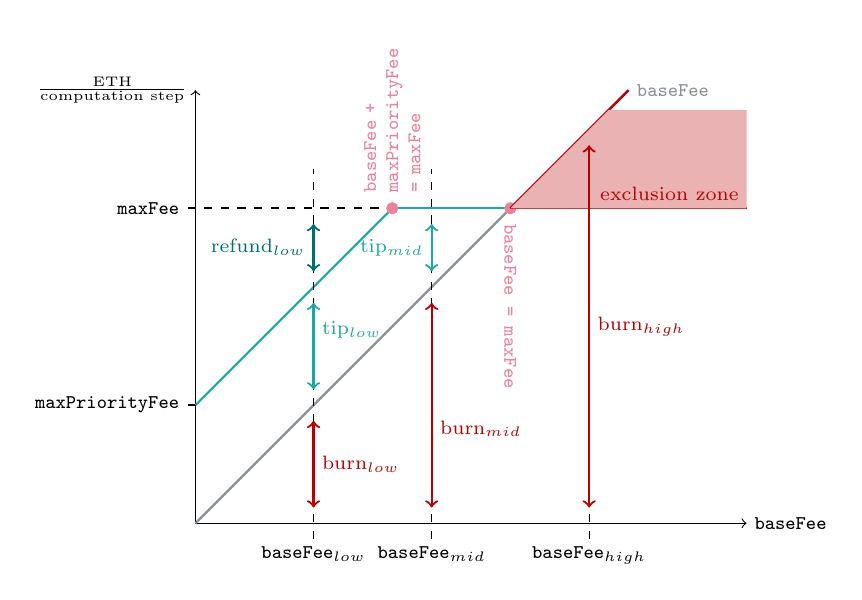
\begin{tikzpicture}

	\scriptsize
	
	%%% axes and 45 degree line
	% axes
	\draw[->] (0,0) -- (7,0) node[right]{\texttt{baseFee}};
	\draw[->] (0,0) -- (0,5.5) node[left]{$\frac{\text{ETH}}{\text{computation step}}$};
	
	% baseFee
	\draw[thick, softanthracite] (0,0) -- (5.5,5.5) node[right]{\texttt{baseFee}};
	
	%%% user-chosen parameters
	\uncover<2->{
	
		% maxFee
		\draw[dashed, thick] (-0.1,4) node[left]{\texttt{maxFee}} -- (7,4);

		% maxPriorityFee
		\draw[dashed, thick] (-0.1,1.5) node[left]{\texttt{maxPriorityFee}} -- (0.1,1.5);
		\draw[thick, color = strongmint] (0,1.5) -- (2.5,4);
		\draw[thick, color = strongmint] (2.5,4) -- (4,4);
	
	}
	
	%%% baseFee "low"
	% vertical line
	\uncover<3-4>{
		\draw[dashed] (1.5, -0.2) node[below]{\texttt{baseFee}$_{low}$} -- (1.5,4.5);
	}
	
	% burn
	\uncover<4-4>{
		\draw[thick, <->, color = focus] (1.5,0.2) -- (1.5,1.3) node[midway, right]{burn$_{low}$};
	
	% tip
		\draw[thick, <->, color = strongmint] (1.5,1.7) -- (1.5,2.8) node[midway, right, yshift=2mm]{tip$_{low}$};
	
	% refund
		\draw[thick, <->, color = darkmint] (1.5,3.2) -- (1.5,3.8) node[midway, left] {refund$_{low}$};
	}
	
	%%% baseFee "mid"
	% vertical line
	\uncover<5-6>{
		\draw[dashed] (3, -0.2) node[below]{\texttt{baseFee}$_{mid}$} -- (3,4.5);
	}
	
	\uncover<6-6>{
	
		% 
		\filldraw[color = softred] (2.5,4) circle (2pt) node[right, yshift=1mm, rotate = 90, text width = 2cm] {\texttt{baseFee + maxPriorityFee = maxFee}};
		% burn
		\draw[thick, <->, color = focus] (3,0.2) -- (3,2.8) node[midway, right, yshift=-3mm]{burn$_{mid}$};
		
		% tip
		\draw[thick, <->, color = strongmint] (3,3.2) -- (3,3.8) node[midway, left]{tip$_{mid}$};
	}

	%%% baseFee "high"
	% vertical line
	\uncover<7-8>{
		\draw[dashed] (5, -0.2) node[below]{\texttt{baseFee}$_{high}$} -- (5,5);
	}
	
	% burn
	\uncover<8-8>{
		\filldraw[color = softred] (4,4) circle (2pt) node[right, yshift=-1mm, rotate = 270] {\texttt{baseFee = maxFee}};
		
		% exclusion zone
		\draw[thick, color = focus] (4,4) -- (7,4);
		\draw[thick, color = focus] (4,4) -- (5.5,5.5);
		\draw[fill=focus!30, draw = none] plot[smooth, samples=100, domain=4:5.25] (\x, \x) -| (7,4) node[above left]{\textcolor{focus}{exclusion zone}} -- cycle;

		% burn
		\draw[thick, <->, color = focus] (5,0.2) -- (5,4.8) node[midway, right]{burn$_{high}$};
	}
	
\end{tikzpicture}
	\end{figure}
	
	\vspace{-1.25em}
	
	\uncover<3->{
	\scriptsize
	\textbf{Three cases:}
	\begin{enumerate}
		\item<3-> \textbf{Refund:} \texttt{baseFee} $+$ \texttt{maxPriorityFee} $<$ \texttt{maxFee}
		\item<5-> \textbf{Partial Tip:} \texttt{baseFee} $+$ \texttt{maxPriorityFee} $\geq$ \texttt{maxFee} \& \texttt{baseFee} $\leq$ \texttt{maxFee}
		\item<7-> \textbf{Pending:} \texttt{baseFee} $>$ \texttt{maxFee}
	\end{enumerate}
	}
	
\end{frame}
%%%

%%%
\begin{frame}{Ethereum Gas Fees: EIP-1559 Base Fee Adjustment}
	\textbf{EIP-1559 Base Fee Adjustment Mechanism}\footnote{\href{https://timroughgarden.org/papers/eip1559.pdf}{Roughgarden (2020) \link}}
	\begin{itemize}
		\item Target block size: currently 15 million gas ($s_{target}$)
		\item Block limit: currently 30 million gas (2x target block size)
		\item Block size and base fee of previous block ($s_{pred}, r_{pred}$) determine base fee of current block ($r_{cur}$):\\
		\vspace{0.5cm}
		$r_{cur} := r_{pred}\cdot\left(1+\frac{1}{8}\cdot\frac{s_{pred}-s_{target}}{s_{target}}\right)$
	\end{itemize}
\end{frame}
%%%

%%%
\begin{frame}{Essential Tools: Ethereum Gas Tracker}
	\begin{figure}
	\centering
	\begin{minipage}{.45\textwidth}
  		\centering
  		\includegraphics[width=0.9\textwidth]{../assets/images/Etherscan.png}
  		\caption*{\footnotesize \href{https://etherscan.io/}{\link Etherscan}}
	\end{minipage}
	\begin{minipage}{.45\textwidth}
  		\centering
  		\includegraphics[width=0.9\textwidth]{../assets/images/ethGasStation.png}
  		\caption*{\footnotesize \href{https://www.Ethgasstation.info}{\link Eth Gas Station}}
	\end{minipage}
	\end{figure}
\end{frame}
%%%

%%%
\begin{frame}{Exercise 1 - Transactions With EIP-1559}
	\begin{exercise}{Exercise 1} 
	For the following questions assume a \texttt{baseFee}  of 0.000000013 GWEI and a threshold \texttt{priorityFee} of 1 GWEI:\footnote{Please note: The values we use in this exercise have been chosen with Ropsten testnet in mind. The Mainnet \texttt{baseFee} is much higher.}
	\begin{enumerate}[a]
		\item Use your Metamask account to initiate a simple ETH value transaction with a \texttt{maxPriorityFee} of 2 GWEI and a \texttt{maxFee} of 3 GWEI. How large do you expect the fee to be considering a gasLimit of 21000?
		\item Use your Metamask account to initiate a simple ETH value transaction with a \texttt{maxPriorityFee} of 0.5 GWEI, a \texttt{maxFee} of 1 GWEI and a gasLimit of 21000. What do you expect to happen?
		\item Use your Metamask account to initiate a simple ETH value transaction with a \texttt{maxPriorityFee} of 2 GWEI, a \texttt{maxFee} of 3 GWEI and a gasLimit of 1000000. What do you expect to happen?
		\item Use your Metamask account to initiate a simple ETH value transaction with a \texttt{maxPriorityFee} of 2 GWEI, a \texttt{maxFee} of 3 GWEI and a gasLimit of 1000. What do you expect to happen?
		\item Use your Metamask account to initiate a simple ETH value transaction with a \texttt{maxPriorityFee} of 3 GWEI, a \texttt{maxFee} of 3 GWEI and a gasLimit of 21000. What do you expect to happen?
	\end{enumerate}
	\end{exercise}
\end{frame}
%%%

%%%
\begin{frame}{Recommended Reading}
\begin{columns}
	\begin{column}{0.3\textwidth}
	\center
	\includegraphics[width=0.5\textwidth , frame]{../assets/images/Roughgarden_cover.png}
	\end{column}
	\begin{column}{0.7\textwidth}
	\textbf{Transaction Fee Mechanism Design for the Ethereum Blockchain: An Economic Analysis of EIP-1559} \\
	Tim Roughgarden, 2020 \\
	\link \href{https://timroughgarden.org/papers/eip1559.pdf}{Online PDF}
	\end{column}
\end{columns}
\begin{columns}
	\begin{column}{0.3\textwidth}
	\center
	\includegraphics[width=0.5\textwidth , frame]{../assets/images/eip_1559_cover.png}
	\end{column}
	\begin{column}{0.7\textwidth}
	\textbf{EIP-1559 FAQ} \\
	Vitalik Buterin, 2021 \\
	\link \href{https://notes.ethereum.org/@vbuterin/eip-1559-faq}{Online PDF}
	\end{column}
\end{columns}
\end{frame}
%%%

\end{document}